\documentclass[12pt]{exam}
\newcommand{\hwnumber}{10}
\newcommand{\hwname}{Huffman Compression}
\newcommand{\duedate}{\formatdate{18}{11}{\YEAR} by \progDueTime} % day-month-year

\newcommand{\C}[1]{\bgroup\fboxsep=1pt\colorbox{Gray!25}{\tt$\!$#1$\!$}\egroup}

\usepackage{../misc/latex/edition}  % Course semester
\usepackage{../misc/latex/c0}       % Listings style for c0
\usepackage{amsmath}
\usepackage{enumerate}
\usepackage[normalem]{ulem}
\usepackage{verbatim}
\usepackage[left=1in, right=1in, top=1in, bottom=1in]{geometry}
\usepackage{graphicx}
\usepackage{hyperref}
\usepackage{tikz}     \usetikzlibrary{shapes}
\usepackage{fancybox}
\usepackage[all]{xy}
\usepackage{wrapfig}
\usepackage{fancyvrb}
\usepackage{datetime}
\usepackage{etoolbox}
\usepackage{calc}
\usepackage[nomessages]{fp}
\usepackage{import}  % Like input and include, but respects subdirectories

\newcommand{\defaultQuestionLocation}{questions}
\newcommand{\inputQuestion}[2][\defaultQuestionLocation/]{%
  \subimport{#1}{#2}
}
% Subdirectories of \defaultQuestionLocation containing code and pictures
\newcommand{\code}{code}
\newcommand{\img}{img}


%%% ic: frontmatter macros
\newcommand{\specialInstructions}{}
\newcommand{\HWNUMBER}
{\ifdefempty{\hwnumber}{__}{%
  \ifnumless{\hwnumber}{10}{0\hwnumber}{\hwnumber}}}
\newcommand{\hwtype}{Written Homework}

%%% ic: 'exam' tweaks
\renewcommand{\half}{.5} % Half points

\newcommand{\Question}[2][]
 {\ifstrempty{#1}
    {\question{\bf #2}}
    {\question[#1]{\bf #2}}
  \immediate\write\rubricfile{}%
  \immediate\write\rubricfile{Question \thequestiontitle:}%
  \immediate\write\rubricfile{==========}
 }

%%% ic: Support for editable PDF
% counter name (some viewers misbehave if always the same)
\newcounter{editable}
\newcommand{\nextField}{\addtocounter{editable}{1}q\arabic{editable}}
\newcommand{\NextField}
 {\makebox[0pt][r]{\scalebox{0.1}{\color{White}\nextField}}}

% Color of edit area
\newcommand{\editAreaColor}{red}
% Single line answer:   \editableLine[extra parameters (optional)]{line width}
\newcommand{\editableLine}[2][]
{\textcolor{\editAreaColor}{%
 \underline{\hspace*{-0.25em}%
 \raisebox{-0.5ex}{%
 \TextField[width=#2, borderwidth=0, #1]{\NextField}}}}%
}
% Single line answer for code:  \editableLine[extra parameters (optional)]{line width}
\newcommand{\editableCodeLine}[2][]
{\textcolor{\editAreaColor}{%
 \underline{%
 \TextField[width=#2, height=1.5ex, borderwidth=0, #1]{\NextField}}}}
% Multiline answer:  \editableLine[extra parameters (optional)]{box height}
\newcommand{\editableBox}[2][]
{\leavevmode\hspace*{-0.1em}%
\TextField[height=#2, width=\linewidth,
           multiline=true, borderwidth=0.1, bordercolor=\editAreaColor,
           #1]{\NextField}}

%%%%% Same answer format as exams
\renewcommand{\rmdefault}{ppl}
\renewcommand{\sfdefault}{phv}
\newcommand{\answerColor}{Blue}

\ifprintanswers
\newcommand{\answer}[2]{\makebox[#1][c]{\color{\answerColor}#2}}
\else
\newcommand{\answer}[2]{\makebox[#1][c]{}\makebox[0pt]{\phantom{|}}}
\fi
\newcommand{\uanswer}[2]{\underline{\answer{#1}{#2}}}


%%% Write rubric snippet.  Usage:
% \RUBRIC
% any multi-line text (including \, #, %, whatever)
% ENDRUBRIC
%% (ENDRUBRIC should be on a line by itself)
\makeatletter
\def\RUBRIC
 {%
  \begingroup
  \let\do\@makeother\dospecials
  \endlinechar=`\^^J
  \@tofile%
 }
\def\ENDRUBRIC{ENDRUBRIC}
\def\@tofile#1^^J{%
  \def\@test{#1}%
  \ifx\@test\ENDRUBRIC
    \immediate\write\rubricfile{}  % End with an empty line
    \expandafter\@firstoftwo
  \else
    \expandafter\@secondoftwo
  \fi
  {\endgroup}%
  {\toks@{#1}%
   \begingroup\endlinechar=\m@ne
   \everyeof{\noexpand}%
   \xdef\@temp{\scantokens\expandafter{\the\toks@}}%
   \endgroup
   \immediate\write\rubricfile{\@temp}%
   \@tofile}%
}
\makeatother

%% Displays tags for an exercise in 'answer' mode
\newcommand{\TAGS}[1]
{\ifprintanswers%
  \rule{0em}{0ex}%
  \marginpar{\footnotesize%
    \fcolorbox{black}{Gray!25}{%
      \parbox[t]{2cm}{\raggedright\textbf{TAGS:}\\#1}}}%
  \ignorespaces%
 \fi}%


%% Page layout
\pagestyle{headandfoot}

\headrule
\header{\textbf{\courseNumber{} \hwtype{} \hwnumber}}
       {}
       {\textbf{Page \thepage\ of \numpages}}
\footrule
\footer{}{}{\COPYRIGHT}

\renewcommand{\partlabel}{\textbf{\thequestion.\thepartno}}
%\renewcommand{\partlabel}{\textbf{Task \thepartno}}
\renewcommand{\subpartlabel}{\textbf{\thesubpart.}}
\renewcommand{\thepartno}{\arabic{partno}}
\renewcommand{\thesubpart}{\alph{subpart}}
\pointpoints{pt}{pts}
\pointformat{\raisebox{0ex}[\height][0pt]{\fcolorbox{black}{yellow}{\themarginpoints}}}
\bonuspointformat{\raisebox{0ex}[\height][0pt]{\fcolorbox{black}{red}{\themarginpoints}}}
\marginpointname{\points}
\pointsinmargin
%\boxedpoints

\setlength\answerlinelength{2in}
\setlength\answerskip{0.3in}

\newcommand{\mkWrittenTitle}[1]{#1}
\newcommand{\mkDueDate}[1]{#1}
\newcommand{\mkEvalSummary}[1]{#1}
\newcommand{\mkGradetable}[1]{#1}



% This fixes an issue with the exam package version 2.6 and after,
% where 'framed' has been renamed to 'examframed' to avoid a conflict.
\ifcsmacro{examframed}{%
\newenvironment{framed}
{\begin{examframed}}
{\end{examframed}}
}{}

\begin{document}
\hwTitle

\noindent
In this programming assignment, we will progressively develop a C
program to compress (and uncompress) files --- something similar to
applications like \lstinline'pkzip'/\lstinline'pkunzip' or
\lstinline'gzip'/\lstinline'gunzip' which you may have used.  Like
these applications, your program will be able to handle inputs as short
as a tweet and as long as the collected works of William Shakespeare,
and it won't be limited to just text files.  Along the way, we will
see how trees can play a role in data compression and why they need to
be supplemented with other data structures to achieve good
performance.  We will also take a quick peek at file input/output in
C\@.

\bigskip
\noindent
The code handout for this assignment is at
\begin{center}
\whereisthetgz{huffman-handout.tgz}
\end{center}
The file \lstinline'README.txt' in the code handout goes over the
contents of the handout and explains how to hand the assignment in.
There is a TEN (10) PENALTY-FREE HANDIN LIMIT.  Every additional
handin will incur a small (5\%) penalty (even if using a late day).

\bigskip
\paragraph{Notes:}
\begin{itemize}
\item%
  This assignment will not be graded for style.  However you will find
  it helpful to apply the good style habits you have developed:
  reasonable contracts, at most 80-character lines, and comments that
  make it clear to a reader how your algorithm works and what
  invariants you expect to hold. You should use the libraries provided
  for you to make your code simple and clear. We expect you to write
  your own helper functions when appropriate.  Bad style will have no
  direct effect on your grade but will make your life harder.
\item%
  Be sure to include appropriate \lstinline"REQUIRES",
  \lstinline"ENSURES", and \lstinline"ASSERT" annotations in your
  code.  If you write any auxiliary functions, include precise and
  appropriate pre- and post-conditions.  You should write these as you
  are writing the code rather than after you're done: documenting your
  code as you go along will help you reason about what it should be
  doing, and thus help you write code that is both clearer and more
  correct.
\item%
  Be careful that all the memory you allocated is freed by the end of
  a normal execution (you do not need to do so for abnormal exits,
  like when encountering an error condition or a contract violations).
  We will use \lstinline'valgrind' to check for memory leaks and
  safety violations \ldots $\,$and so should you.
\end{itemize}


\clearpage
\section*{Data Compression: Overview}

Whenever we represent data in a computer, we have to choose some sort
of \emph{encoding} with which to express it in binary.  When
representing strings in C0, for instance, we use ASCII codes to
represent the individual characters.  Other encodings are possible as
well.  For example, the UNICODE standard defines several character
encodings with a variety of different properties.  The simplest,
UTF-32, uses 32 bits per character.

Under the extended ASCII encoding, each character is represented using
8 bits, so a string of length $n$ requires $8n$ bits of storage.  For
example, consider the string \lstinline'"free coffee"'.  It is
represented as the following $11 \times 8 = 88$ bits in ASCII:
\begin{center}\tt
\newcommand{\g}[1]{\textcolor{\stringColor}{#1}}
\begin{tabular}{*{11}{l}}
  01100110 & 01110010 & 01100101 & 01100101 & 00010000 & 01100011 & 01101111
\\\g{f}    & \g{r}    & \g{e}    & \g{e}    & \g{ }    & \g{c}    & \g{o}
\\[2ex]
  01100110 & 01100110 & 01100101 & 01100101
\\\g{f}    & \g{f}    & \g{e}    & \g{e}
\end{tabular}
\end{center}
(The spaces around the ASCII code of each letter are shown to ease
readability: they are not part of the encoding of this string.  Also,
\lstinline'00010000' is the ASCII code of the space character.)

%Sometimes when we wish to store a large quantity of data, or to transmit a
%large quantity of data over a slow network link, it may be advantageous to
%seek a specialized encoding that requires less space to represent our data
%by taking advantage of redundancies inherent in it.

This encoding of the string is rather wasteful, though.  In fact,
since there are only 6 distinct characters in the string (including
the space character), we should be able to represent it using a custom
encoding that uses only $\lceil \log 6 \rceil = 3$ bits to represent
each character.  If we were to use the following custom encoding:
\begin{center}
\newcommand{\g}[1]{\textcolor{\stringColor}{\lstinline"'"{\tt #1}\lstinline"'"}}
\begin{tabular}{cc}
   \textbf{Character} & \textbf{Code}
\\\hline \\[-1ex]
   \g{c}              & \tt 000
\\ \g{e}              & \tt 001
\\ \g{f}              & \tt 010
\\ \g{o}              & \tt 011
\\ \g{r}              & \tt 100
\\ \g{ }              & \tt 101
\end{tabular}
\end{center}
the string would be represented with only $11 \times 3 = 33$ bits:
\begin{center}\tt
\newcommand{\g}[1]{\textcolor{\stringColor}{#1}}
\begin{tabular}{@{}*{16}{l}@{}}
  010   & 100   & 001   & 001   & 101   & 000   & 011   & 010   & 010   & 001   & 001
\\\g{f} & \g{r} & \g{e} & \g{e} & \g{ } & \g{c} & \g{o} & \g{f} & \g{f} & \g{e} & \g{e}
\end{tabular}
\end{center}
By using this custom encoding, we have saved $(88 - 33) / 88 = 62\%$
of the space used by the standard ASCII representation of the
above string.\footnote{Well, almost: we would also need to store the
  encoding itself so that we can recover the string --- more on this
  later.}

Can we do even better?  Our custom encoding uses the same number of
bits for each character --- it is a \emph{fixed-length encoding}.  But
in our input string, the letter \textcolor{\stringColor}{\tt e} occurs
much more frequently than \textcolor{\stringColor}{\tt c} for
instance.  It may be worthwhile to use a smaller bit pattern to encode
the character \textcolor{\stringColor}{\tt e} even at the expense of
having to use longer bit patterns to encode
\textcolor{\stringColor}{\tt c}.  Our next encoding --- a
\emph{variable-length encoding} --- embraces this idea:
\begin{center}
\label{tab:hcode}
\newcommand{\g}[1]{\textcolor{\stringColor}{\lstinline"'"{\tt #1}\lstinline"'"}}
\begin{tabular}{cc}
   \textbf{Character} & \textbf{Code}
\\\hline
\\ \g{c}              & \tt 1101
\\ \g{e}              & \tt 0
\\ \g{f}              & \tt 10
\\ \g{o}              & \tt 1110
\\ \g{r}              & \tt 1111
\\ \g{ }              & \tt 1100
\end{tabular}
\end{center}
Using it, the string \lstinline'"free coffee"' is represented as follows:
\begin{center}\tt
\newcommand{\g}[1]{\textcolor{\stringColor}{#1}}
\begin{tabular}{@{}*{16}{l}@{}}
  10    & 1111  & 0     & 0     & 1100  & 1101  & 1110  & 10    & 10    & 0     & 0
\\\g{f} & \g{r} & \g{e} & \g{e} & \g{ } & \g{c} & \g{o} & \g{f} & \g{f} & \g{e} & \g{e}
\end{tabular}
\end{center}
That's just 26 bits, for a $(88 - 26)/88 = 70\%$ space saving.

For a variable-length encoding to be viable, there needs to be a
simple way to go from a bit string like the above to the original
text.  One such way is for the encoding to be \emph{prefix-free}: no
code word is a prefix of any other code word.  Both our encodings are
prefix-free: in the last one, for example, if a bit string starts with
\lstinline'10', the first character of the corresponding text must be
\textcolor{\stringColor}{\tt f} because no other character encoding
starts with \lstinline'10'.

It can be proven that this encoding is optimal for this particular
string: no other prefix-free encoding can represent the string using
fewer than 26 bits.  Moreover, the encoding is optimal for \emph{any}
string that has the same distribution of characters as the sample
text.  In this assignment, you will implement a method for
constructing such optimal encodings developed by David Huffman.

\subsection*{Huffman Coding: A Brief History}

\emph{Huffman coding} is an algorithm for constructing optimal
prefix-free encodings given a frequency distribution over characters.
It was developed in 1951 by David Huffman when he was a Ph.D student
at MIT taking a course on information theory taught by Robert Fano.
It was towards the end of the semester, and Fano had given his
students a choice: they could either take a final exam to demonstrate
mastery of the material, or they could write a term paper on something
pertinent to information theory.  Fano suggested a number of possible
topics, one of which was efficient binary encodings: while Fano
himself had worked on the subject with his colleague Claude Shannon,
it was not known at the time how to efficiently construct optimal
encodings.

Huffman struggled for some time to make headway on the problem and was
about to give up and start studying for the final when he hit upon a key
insight and invented the algorithm that bears his name, thus outdoing his
professor, making history, and attaining an ``A'' for the course.  Today,
Huffman coding enjoys a variety of applications: it is used as part of the
DEFLATE algorithm for producing ZIP files and as part of several multimedia
codecs like JPEG and MP3.


\clearpage
\section{Huffman Trees}
\label{sec:tree}

Prefix-free encodings --- where no code word is a prefix of any other
code word --- can be represented as binary trees with characters
stored at the leaves: a branch to the left corresponds to a 0 bit and
a branch to the right corresponds to a 1 bit, so that the path from
the root to a leaf gives the code word for the character stored at
that leaf.

For instance, the fixed-length and variable-length encodings shown
earlier --- both being prefix-free --- are represented by the
following two binary trees, respectively.

\bigskip
\noindent
\begin{minipage}[t]{0.5\textwidth}
\begin{raggedleft}
\raisebox{1.6cm}{%
  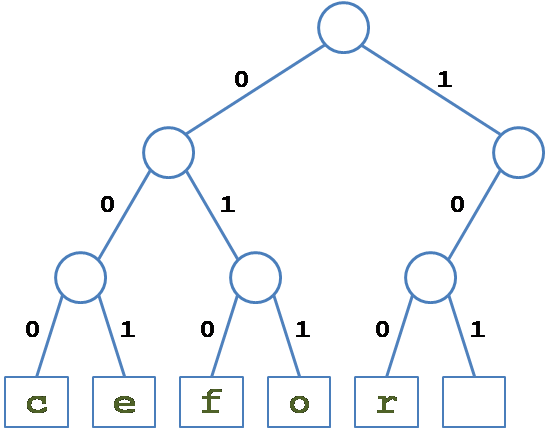
\includegraphics[width=0.87\linewidth]{\img/fixed.png}}
\end{raggedleft}
\end{minipage}%
\hfill\rule{0em}{7cm}%
\begin{minipage}[t]{0.5\textwidth}
\begin{raggedright}
  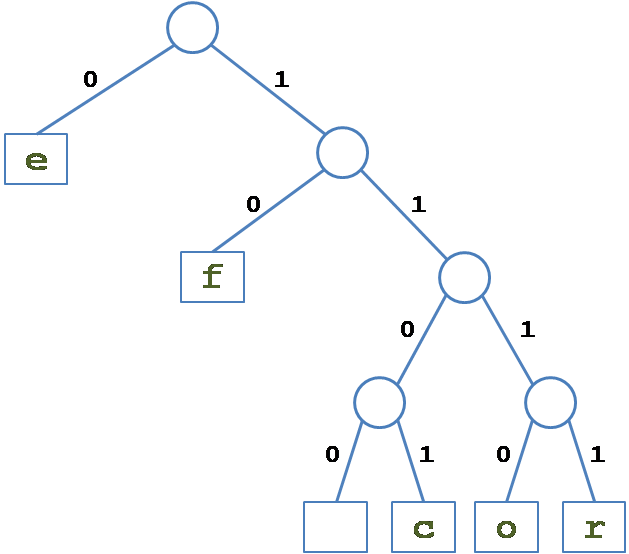
\includegraphics[width=1.0\linewidth]{\img/variable.png}
\end{raggedright}
\end{minipage}

In the tree on the right, which corresponds to our variable-length
encoding, frequently-occurring characters have shorter paths from the
root.  We can see this property clearly if we label each subtree with
the total frequency of the characters occurring at its leaves.  The
frequencies in the following tree are based on the sample string
\lstinline'"free coffee"'.  A frequency-annotated tree is called a
\emph{Huffman tree}.

\enlargethispage{5ex}
\begin{center}
  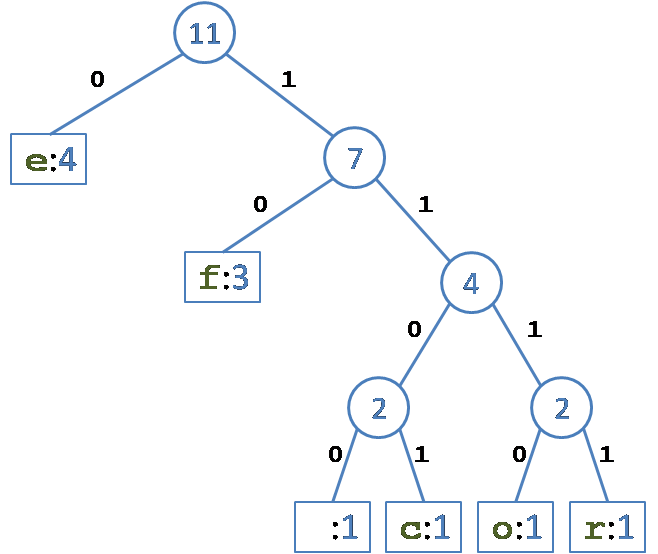
\includegraphics[width=0.6\textwidth]{\img/htree.png}
\end{center}

Huffman trees have a recursive structure: a Huffman tree is either a
leaf containing a character and its frequency, or an interior node
containing the combined frequency of two child Huffman trees.  We draw
the leaves, which contain character data, as rectangles to distinguish
them from the interior nodes, which we draw as circles.

We represent both kinds of Huffman tree nodes in C using a
\lstinline'struct htree_node', abbreviated as the type \lstinline'htree':
\begin{lstlisting}
  typedef struct htree_node htree;
  struct htree_node {
    symbol_t value;
    unsigned int frequency;
    htree *left;
    htree *right;
  };
\end{lstlisting}
The \lstinline'value' field of a leaf contains a character and is
irrelevant for interior nodes.  Interior nodes should have exactly two
children.  In view of generalizing our encoding from strings of
printable characters to arbitrary data, we draw \lstinline'value' from
the type \lstinline'symbol_t' of \emph{symbols}.  \lstinline'symbol_t'
is an unsigned integer type, making it suitable to index arrays by
symbols.  Within this type, the symbols we may want to represent are
in the range $[0, \lstinline'NUM_SYMBOLS')$.

The well-formedness criteria of Huffman trees give rise to the
following recursive definitions:
\begin{itemize}
\item%
  An \lstinline'htree' is a \emph{valid htree} if it is
  non-\lstinline'NULL' and it is either a \emph{valid htree leaf} or a
  \emph{valid htree interior node}.
\item%
  An \lstinline'htree' is a \emph{valid htree leaf} if its
  \lstinline'frequency' is strictly positive, and
  \lstinline'left' and \lstinline'right' children are
  \lstinline'NULL'.
\item%
  An \lstinline'htree' is a \emph{valid htree interior node} if its
  \lstinline'left' and \lstinline'right' children are \emph{valid
    htrees}, and its \lstinline'frequency' is the sum of the
  \lstinline'frequency' of its children.
\end{itemize}

\begin{task}[2]
\TAGS{ds-invariant, pointer, struct}
In file \lstinline'huffman.c', implement the following functions that
formalize the Huffman tree data structure invariants:
\begin{center}
\begin{tabular}{l@{\hspace{3em}}l}
\textbf{Function:}                            & \textbf{Returns \lstinline'true' iff...}
\\[1ex]
   \lstinline"bool is_htree_leaf(htree *H);"     & the node is a leaf
\\ \lstinline"bool is_htree_interior(htree *H);" & the node is an interior node
\\ \lstinline"bool is_htree(htree *H);"          & the tree is a Huffman tree
\end{tabular}
\end{center}
\end{task}

You may test your code by hand-building various \lstinline'htree''s
in file \lstinline'test-htree.c'.  Compile your work with
\begin{lstlisting}
# make htree
\end{lstlisting}
and then run your tests with
\begin{lstlisting}
# ./test-htree
\end{lstlisting}
The next tasks will further exercise your specification functions.


\section{Constructing Huffman Trees}
\label{sec:build}

\begin{figure}[p]
\enlargethispage{3ex}
\centering
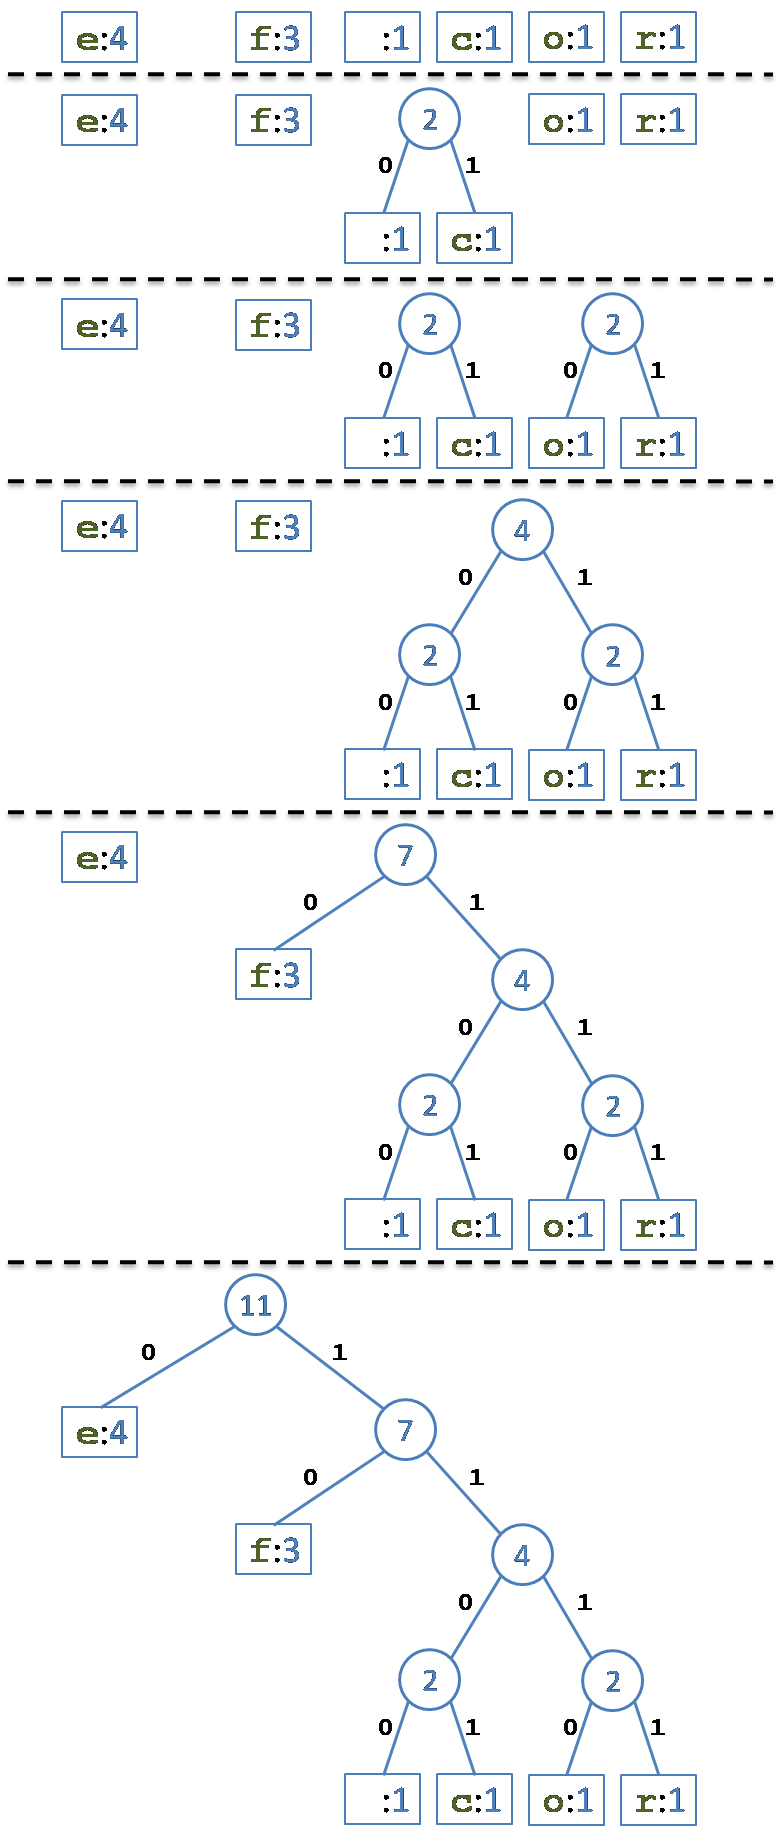
\includegraphics[height=1.02\textheight]{\img/build-htree.png}
\label{fig:htree-build}
\end{figure}

Huffman's key insight was to use the frequencies of symbols to build an
optimal encoding tree from the bottom up.  Given a set of symbols and
their associated frequencies, we can build an optimal Huffman tree as
follows:
\begin{enumerate}
\item%
  Construct leaf Huffman trees for each symbol/frequency pair.
\item\label{step:loop}%
  Repeatedly choose two minimum-frequency Huffman trees and join
  them together into a new Huffman tree whose frequency is the sum
  of their frequencies.
\item%
  When only one Huffman tree remains, it represents an optimal
  encoding.
\end{enumerate}
This is an example of a \emph{greedy algorithm} since it makes locally
optimal choices that nevertheless yield a globally optimal result at
the end of the day.  Selection of a minimum-frequency tree in step
\ref{step:loop} can be accomplished using a \emph{priority queue}
based on a heap.  A sample run of the algorithm is shown on
page~\pageref{fig:htree-build}.

\begin{task}[5]
\TAGS{c-array, ds-invariant, interface, pointer, pq}
In file \lstinline'huffman.c', write a function
\begin{lstlisting}
  htree* build_htree(freqtable_t table);
\end{lstlisting}
that constructs an optimal encoding for an alphabet with
\lstinline'NUM_SYMBOLS' symbols using Huffman's algorithm.  The
\emph{frequency table} \lstinline'table', of type
\lstinline'freqtable_t', is an unsigned integer array of length
\lstinline'NUM_SYMBOLS'.  The entry \lstinline'table[c]' contains the
reported frequency of symbol \lstinline'c', which may be 0 if
\lstinline'c' is not expected to occur in a text (for example if
\lstinline'c' is a non-printable ASCII character and we are only
interested in encoding text files).  See file \lstinline'freqtable.h'.

Use the code in the included \lstinline'lib/heaps.c' as your
implementation of priority queues.
\end{task}

Two observations:
\begin{itemize}
\item%
  Huffman trees for a frequency table with just one symbol are not
  particularly useful, because the optimal encoding of a single symbol
  would be the empty bit string.  But the source strings, all of
  which must just repeat the same symbol, would be mapped to the same
  empty string.  Therefore, \lstinline'build_htree' must signal an
  error (by calling the \lstinline'error' function) if there are fewer
  than two symbols with non-zero frequency, and otherwise return an
  interior node as a result.
\item%
  Huffman trees are not unique due to symmetries, additionally
  complicated by the fact that multiple symbols or subtrees might have
  identical frequencies.  All possible valid Huffman codes for a given
  text will have the same length (due to its optimality guarantee) but
  may otherwise be different.  So the particular codes produced in
  your implementation may look different from the ones shown in this
  writeup.
\end{itemize}
The directory \lstinline'data/freq' contains a number of frequency files,
which have a textual representation format
\begin{lstlisting}
    [*\C{<symbol 1>}*]:[*\C{<frequency 1>}*]
    [*\C{<symbol 2>}*]:[*\C{<frequency 2>}*]
    ...
\end{lstlisting}
where the symbol is separated from the frequency by a colon
\lstinline"':'".  Each \C{\lstinline'<symbol n>'} is either a printable
ASCII character (like \lstinline'A') or an hexadecimal number of the
form \lstinline'0x'$nn$ (like \lstinline'0x41').  By convention,
frequency files have a \lstinline'.frq' extension.  Take a look the
frequency file for our ongoing example at
\lstinline'data/freq/free_coffee.frq'.

You can test your implementation by compiling your code with
\begin{lstlisting}
# make
\end{lstlisting}
and then running
\begin{lstlisting}
# ./huff-safe -f [*\C{<freq\_file>}*] -R
\end{lstlisting}
The command-line flag \lstinline'-R' instructs \lstinline'huff-safe'
to print the \lstinline'htree' it has built from frequency file
\C{\lstinline'<freq_file>'}.  Use the additional flag \lstinline'-Q' to
also display the frequency table in \C{\lstinline'<freq_file>'}.

For instance, to test your code with our
ongoing example, you would type:
\begin{lstlisting}
# ./huff-safe -f data/freq/free_coffee.frq -R
\end{lstlisting}
or, if you want to display the frequency table,
\begin{lstlisting}
# ./huff-safe -f data/freq/free_coffee.frq -R -Q
\end{lstlisting}


\section{Decoding Bit Strings}
\label{sec:decode}

The Huffman encoding of a text using a Huffman tree that accounts for
all of the symbols in it is a bit string that replaces each symbol
with its Huffman code.  We will see how to efficiently carry out such
encoding shortly.  One thing we can do right away is decode a bit
string using the very Huffman tree that was used to encode it.

Given an encoded bit string and the Huffman tree that was used to
encode it, we decode the bit string as follows:
\begin{enumerate}
\item%
  Initialize a pointer to the root of the Huffman tree.
\item%
  Repeatedly read bits from the bit string and update the pointer:
  when you read a 0, follow the left branch, and when you read a 1,
  follow the right branch.
\item%
  Whenever you reach a leaf, output the symbol at that leaf and reset
  the pointer to the root of the Huffman tree.
\end{enumerate}
If the bit string was properly encoded, then when all of the bits are
exhausted, the pointer should once again point to the root of the
Huffman tree.  If this is not the case, then the decoding fails for
the given input.

As an example, we can use our on-going encoding to decode the
following message:
\begin{center}\tt
\newcommand{\g}[1]{\textcolor{\stringColor}{#1}}
\begin{tabular}{*{40}{@{$\:$}r}}
  1&1&0&1   &1&1&1&0  &1&0    &1&0    &0     &0     &1&1&0&0  &1&0    &1&1&1&0  &1&1&1&1  &1&1&0&0  &1&0    &1&1&1&1  &0     &0
\\ &&&\g{c} &&&&\g{o} &&\g{f} &&\g{f} &\g{e} &\g{e} &&&&\g{ } &&\g{f} &&&&\g{o} &&&&\g{r} &&&&\g{}  &&\g{f} &&&&\g{r} &\g{e} &\g{e}
\end{tabular}
\end{center}

\newpage
\begin{task}[8]
\TAGS{c-array, ds-invariant, pointer, string}
In file \lstinline'huffman.c',  implement the decode function
\begin{lstlisting}
symbol_t* decode_src(htree *H, bit_t *code, size_t *src_len);
\end{lstlisting}
This function takes in a bit string \lstinline'code' (details below)
and the Huffman tree \lstinline'H' to decode it with.  It returns an
array of symbols decoded from \lstinline'code' using \lstinline'H'.
The last argument, the pointer \lstinline'src_len', is used by the
function to communicate to the caller the length of the returned
array.  Of the several ways to approach this function, we suggest you
do two passes on the input, one pass to determine the length of the
array to return, and a second pass to populate it.

The function should return the decoded bit string if the string can be
decoded and should signal an error otherwise, using the
\lstinline'error' function.

For your convenience, the bit string \lstinline'code' is a
(\lstinline'NUL'-terminated) C string of the ASCII characters
\lstinline"'0'" and \lstinline"'1'" --- not a great choice for file
compression but good enough for the time being.  We call this
representation of bit strings ``binascii''.
\end{task}

After compiling your code using \lstinline'make', you can test it by
running
\begin{lstlisting}
# ./huff-safe -D -a [*\C{<binascii\_file>}*] -r [*\C{<htree\_file>}*]
\end{lstlisting}
This asks \lstinline'huff-safe' to use your \lstinline'src_decode'
function to decode the binascii string in file
\C{\lstinline'<binascii_file>'} using the Huffman tree in file
\C{\lstinline'<htree_file>'}.  The decoded text will be printed on the
terminal, together with some statistics.  The handout directory
\lstinline'data/binascii' contains sample binascii files with
extension \lstinline'.01'.  Huffman tree files have the format
\begin{lstlisting}
    [*\C{<symbol 1>}*]:[*\C{<Huffman code 1>}*]
    [*\C{<symbol 2>}*]:[*\C{<Huffman code 2>}*]
    ...
\end{lstlisting}
You can find a few Huffman tree files, with extension
\lstinline'.htr', in directory \lstinline'data/htree' (and you can
make your own --- but make sure that they correspond to valid Huffman
trees!).  As usual, you can use the flags \lstinline'-Q' and
\lstinline'-R' to display the frequency table and the Huffman tree if
you wish.  Additionally, the \lstinline'-V' flag will display the
encoded and decoded texts in lockstep for ease of debugging.

Thus, to test your \lstinline'src_decode' on our ongoing example, you
would run
\begin{lstlisting}
# ./huff-safe -D -a data/binascii/free_coffee.01 -r data/htree/free_coffee.htr
\end{lstlisting}
which should result in the string \lstinline'"free coffee"' being
printed on the terminal.


\section{Encoding Strings}
\label{sec:encode}

To encode a text using a Huffman tree appropriate for it, we need to
replace each symbol in it with its Huffman code.  One way to do this
is to traverse the entire tree for each symbol in the text: for a tree
containing $n$ symbols, that's $O(n)$ for each traversal --- check it
out --- so that encoding a text of length $m$ would take $O(nm)$.

A smarter way to proceed is to build an auxiliary data structure that
allows us to retrieve the Huffman code of each symbol in constant time
--- like the table on page~\pageref{tab:hcode}.  We use an array with
\lstinline'NUM_SYMBOLS' entries, each containing the
\lstinline'NUL'-terminated bit string code of one of the symbols (or
\lstinline'NULL' if this symbol is not in our Huffman tree).  A single
traversal of the Huffman tree is sufficient to populate this
\emph{code table}, and from then on a constant-time array access gives
us the Huffman encoding of each input symbol.  The price we pay for
this gain in efficiency is extra memory to store the code table ---
typically a worthy trade-off.

\begin{task}[3]
\TAGS{c-array, ds-invariant, string, traverse-ds}
In file \lstinline'huffman.c', write the function
\begin{lstlisting}
codetable_t htree_to_codetable(htree *H);
\end{lstlisting}
mapping Huffman trees to their code tables.  \emph{Hint: it's pretty
  short done recursively.}  The type
\lstinline'codetable_t', defined in file \lstinline'htree.h', is an
array of (\lstinline'NUL'-terminated) \lstinline'bit_t*'.  This array
has size \lstinline'NUM_SYMBOLS'.
\end{task}
You can test your code by running
\begin{lstlisting}
# ./huff-safe -f [*\C{<freq\_file>}*] -T
\end{lstlisting}
where the flag \lstinline'-T' prints the code table of the Huffman
tree constructed from frequency file \C{\lstinline'<freq_file>'}.
Doing so on our ongoing example takes the form
\begin{lstlisting}
# ./huff-safe -f data/freq/free_coffee.frq -T
\end{lstlisting}

\medskip%
Finally, we are ready to write the encoding function.

\begin{task}[3]
\TAGS{c-array, string}
In the same file, write a function
\begin{lstlisting}
bit_t* encode_src(codetable_t table, symbol_t *src, size_t src_len);
\end{lstlisting}
that efficiently encodes \lstinline'src' of length \lstinline'src_len'
using code table \lstinline'table'.  This function returns the
resulting binascii bit string.  Again, you may want to consider a
two-pass implementation.

The function should return the encoded bit string if the string can be
encoded and should signal an error otherwise, using the
\lstinline'error' function.
\end{task}

You can test your code by running
\begin{lstlisting}
# ./huff-safe -E -s [*\C{<source\_file>}*] -f [*\C{<freq\_file>}*]
\end{lstlisting}
This will use your \lstinline'encode_src' to return the binascii
encoding the file \C{\lstinline'<source_file>'} using frequency file
\C{\lstinline'<freq_file>'}, together with some statistics.  The frequency
file corresponding to sample texts in directory
\lstinline'data/source' have a similar name with a \lstinline'.frq'
extension in directory \lstinline'data/freq'.  Supplying the usual
\lstinline'-Q', \lstinline'-R', \lstinline'-T', and/or \lstinline'-V'
flags will provide additional information were you to need it.  Doing
this on our ongoing example takes the form
\begin{lstlisting}
# ./huff-safe -E -s data/source/free_coffee.txt -f data/freq/free_coffee.frq
\end{lstlisting}
You can save the encoded text by supplying a %
\lstinline'-a '\C{\lstinline'<binascii_file>'}.  If you do so, the
invocation
\begin{lstlisting}
# ./huff-safe -D -a [*\C{<binascii\_file>}*] -f [*\C{<freq\_file>}*]
\end{lstlisting}
should give you back the contents of \C{\lstinline'<source_file>'}.
Try that!


\section{Basic Input/Output in C}
\label{sec:i/o}

Up to now, symbol frequencies are independent from the source files
they are used to encode.  To compress a file the way \lstinline'pkzip'
does it, we need to draw the symbol frequencies from this very file.
This task gives us an opportunity to learn a bit about file
input/output in C\@.  In truth, we will be just scratching the
surface of this far-ranging topic, but we need to start somewhere.

In a C program, we read and write to a file via a \emph{file
  descriptor}, a pointer of type \lstinline'FILE*'.  We obtain a file
descriptor by calling the function \lstinline'fopen(fname, mode)'
where \lstinline'fname' is the path of the file we want to work with,
and \lstinline'mode' is a string with which we tell \lstinline'fopen'
whether we want to read from (\lstinline'"r"') or write to
(\lstinline'"w"') this file.  Once we are done using the file, we need
to close its descriptor using the function \lstinline'fclose(descr)'.

The function \lstinline'fgetc(descr)' reads the next character from the file
with descriptor \lstinline'descr'.  But there may be no next
character if we have reached the end of the file!  In that case it
will return the special value \lstinline'EOF'.

As a summary, here are the (slightly simplified) prototypes of the
above functions:
\begin{lstlisting}
FILE *fopen(char *fname, char *mode);
void fclose(FILE *desc);
int fgetc(FILE *descr);
\end{lstlisting}
You can read more about file I/O in C by researching the library
\lstinline'<stdio.h>'.

\begin{task}[1]
\TAGS{c-array, string, other-types}
In file \lstinline'huffman.c', write the function
\begin{lstlisting}
freqtable_t build_freqtable(char *fname);
\end{lstlisting}
which returns the frequency table of the symbols in file
\lstinline'fname'.
\end{task}
You can test this function by running
\begin{lstlisting}
# ./huff-safe -F -s [*\C{<source\_file>}*]
\end{lstlisting}
For example,
\begin{lstlisting}
# ./huff-safe -F -s data/source/free_coffee.txt
\end{lstlisting}
In fact, you can now test your \lstinline'encode_src' by running
\begin{lstlisting}
# ./huff-safe -E -s [*\C{<source\_file>}*]
\end{lstlisting}
It will use your \lstinline'build_freqtable' to compute the frequency
table of \C{\lstinline'<source_file>'} rather than reading it from a
frequency file.  This is done as follows for our ongoing example:
\begin{lstlisting}
# ./huff-safe -E -s data/source/free_coffee.txt
\end{lstlisting}


\newpage
\section{Packing Bits into Bytes}

Our goal for this assignment is to perform actual file compression,
but binascii uses a whole byte to represent each bit.  Your next task
will be to compress a binascii bit string into actual binary.

\begin{task}[2]
\TAGS{bit-patterns, c-array, string}
In file \lstinline'huffman.c', implement the functions
\begin{lstlisting}
uint8_t* pack(bit_t *bits);
bit_t* unpack(uint8_t *c, size_t len);
\end{lstlisting}
\lstinline'pack(bits)' returns an array of bytes (type
\lstinline'uint8_t') where each \lstinline"'0'" in \lstinline'bits' is
shrunk into a 0-bit and each \lstinline"'1'" into a 1-bit.  The first
digit in \lstinline'bits' will be the most significant bit of the
first byte of the result.  If the size of \lstinline'bits' is not
divisible by 8, the last byte is padded with 0-bits.

Conversely, \lstinline'unpack(bytes, len)' converts each bit in the
byte array \lstinline'bytes' of length \lstinline'len' into a
\lstinline'NUL'-terminated binascii string.
\end{task}
You may find it useful to write helper functions that pack/unpack a
single byte.  Also, the function \lstinline'num_padded_bytes' may come
handy.

We encourage you to write standalone tests for \lstinline'pack' and
\lstinline'unpack', similarly to what you did for \lstinline'is_htree'
in task 1.  This time, we won't give you a starter file for it.

You can test your code thoroughly by performing actual
compression and uncompression on files:
\begin{lstlisting}
# ./huff-safe -C -s [*\C{<source\_file>}*] -h [*\C{<compressed\_file>}*]
\end{lstlisting}
uses the code you have developed in this assignment to compress
\C{\lstinline'<source_file>'} writing the result into
\C{\lstinline'<compressed_file>'}.  This file contains both a code
table extracted from \C{\lstinline'<source_file>'} and the packed
Huffman encoding of its contents.  The compression ratio, i.e., the
space savings, will be printed to terminal.  You can supply the flags
we have encountered so far to display various information.  Thus, to
compress our ongoing example into the file
\lstinline'my_first_compression.hip', you would type
\begin{lstlisting}
# ./huff-safe -C -s data/source/free_coffee.txt -h my_first_compression.hip
\end{lstlisting}

You can use any file you want as the source file, but if you try it
out on very large files, you will want to compile your code with
\lstinline'make fast' and use \lstinline'huff-fast' instead of
\lstinline'huff-safe'.  Do so only after you are sure your code works
properly as it disables all annotations!

You can compress binary files, for example images, but doing so may
not save all that much space --- you may even get a negative
compression ratio since the compressed file embeds the code table of
your source file!

Now the real test.  You can uncompress a compressed file by running
\begin{lstlisting}
# ./huff-safe -U -h [*\C{<compressed\_file>}*]
\end{lstlisting}
to display the corresponding source to terminal.  So, the call
\begin{lstlisting}
# ./huff-safe -U -h my_first_compression.hip
\end{lstlisting}
should print \lstinline'"free coffee"' together with some statistics.

Add the argument \lstinline'-s '\C{\lstinline'<file>'} to dump the
result to \C{\lstinline'<file>'} instead, which will be helpful if the
original source was very large or binary.  The usual flags are
available for your perusal.

For testing purposes, we provide a number of compressed files (with
extension \lstinline'.hip') in directory \lstinline'data/compressed'.
Uncompress them and check that they are identical to the corresponding
source files in directory \lstinline'data/source' by using the Unix
\lstinline'diff' utility.


\section{The Ultimate Test}

How much confidence do you have in your implementation?  Are you
willing to submit your work in \emph{compressed} form?  That's exactly
what you will need to do to get the last point of this assignment.

\begin{task}[1]
\TAGS{correctness}
  Compress your submission, file \lstinline'huffman.c', into a file
  named \lstinline'huffman.c.hip' and submit this file to \autolab{}.

We will use our code to decompress it and then grade what comes out.
If decompression fails, or the result are not a valid C file, you will
get a 0 for the whole assignment.  Don't panic though: if you tested
your code vigorously for all prior tasks and it worked as expected,
the odds of this happening are \emph{very low}.  Moreover, you can
always look at the Autolab output and make a regular submission if it
reports a failed decompression.
\end{task}

\end{document}
